\documentclass[main.tex]{subfiles}

\begin{document}
        \chapter{Le marché monétaire}
        \section{Qu'est ce que la monnaie?}
        \subsection{Dimension politique: symbole de souveraineté}
        Le développement des crypto monnaies, comme le Bit coin, est significatif. Il n'est pas uniquement justifiée par des causes économiques. Le Bit coin est une monnaie dont la valeur fluctue énormément, elle  ne peut servir de \emph{réserve de valeur}, il s'agit d'une monnaie \emph{spéculative}. Sa création provient d'un désir d'avoir une monnaie qui n'est pas gérée par un pouvoir politique, comme la \emph{Banque Centrale}. La conception même de cette monnaie, basée sur une idée de \emph{contrôle mutuel}, l'empêche d'être gérée par un unique pouvoir centralisé.

        \begin{definition}[Réserve de valeur]
                Il s'agit d'une des trois fonctions de la monnaie. La monnaie permet l'épargne, c'est à dire l'accumulation de valeur, ce qui entraine le développement et la croissance au long terme entre autres. Il faut néanmoins pour cela une monnaie \emph{stable}, assujettie à de faibles fluctuations.
        \end{definition}

        \begin{definition}[Banque Centrale]
                La Banque centrale d'un ou de plusieurs pays est une institution chargée par l'État, ou un ensemble d'États dans le cas d’une zone monétaire comme la zone euro, de décider d'appliquer la politique monétaire.
        \end{definition}

La monnaie, à l'origine, a été introduite pour remplacer le \emph{troc} et permettre d'avoir des échanges plus efficaces. Aux origines politiques de la monnaie, en Asie mineure, elle représente le pouvoir royal et permet de payer \emph{le tribu}, les impôts. La fonction d'échange ne se met en place qu'après. Par exemple à Athènes, le revers d'un \emph{tétradrachme} est orné d'une chouette, symbole politique de la ville, la monnaie en circulant fait rayonner le pouvoir de la ville dans les cités soumises. De même en France on retrouve le portrait du roi sur le revers des écus.
        La confiance dans une monnaie est \emph{primordiale}, malgré les grands changements politiques au sein d'un pays la monnaie peut garder son identité, notamment son nom. Par exemple le rouble en Russie change d'aspect après la révolution de 1917 mais le nom est conservé. \\
        La dimension nationale joue aussi un rôle important. L'euro est le seul exemple de monnaie où l'espace de souveraineté monétaire ne correspond pas à l'espace de la souveraineté politique.

        \subsection{Valeur de la monnaie: inverse du niveau des prix}
        \emph{La valeur de la monnaie est l'inverse du niveau des prix.} Si les prix augmentent la monnaie perd de sa valeur, le consommateur perd de son pouvoir d'achat, et inversement. Ceci montre que la question de \emph{l'inflation} est au cœur même de l'idée de monnaie. \\

        \begin{definition}[Inflation]
                Accroissement excessif des instruments de paiement, billets de banque ou capitaux, entraînant une hausse des prix et une dépréciation de la monnaie. Ce concept s'oppose à la déflation.
                Il est bon de noter que plus il y a d'activité économique, moins il y a d'inflation.
        \end{definition}
        On constate depuis les années 80 une tendance globale de faible inflation, voire de déflation. On se propose d'expliquer ce phénomène.

        \begin{definition}[Taux d'intéret directeurs]
        Taux que fixe la banque centrale pour créer de la monnaie à la demande des banques. Lorsqu'une banque veut effectuer un grand prêt par exemple elle doit donner des actifs à la banque centrale qui va créer de la monnaie et lui faire payer des \emph{intérêts directeurs}. Plus ce taux est élevé, plus les taux d'intérêt que les banques pratiquent augmentent, et donc plus les investissements et la consommation diminuent. Cela entraîne donc une baisse de l'activité économique et donc de l'inflation.
        \end{definition}

        On remarque qu'à la fin de l'année 1979 la banque centrale des États Unis décide d'augmenter brutalement les taux d'intérêt directeurs, ce qui casse l'inflation. Une faible inflation est nécessaire pour la mise e place d'un contexte économique \emph{stable}, dans lequel les monnaies ne perdent pas de valeur, au sens énoncé précédemment. Puisque les États Unis étaient alors une puissance économique mondiale, on retrouve une baisse de l'inflation parallèle en Europe. L'inflation suit donc la politique monétaire des banques. \\

        Une autre déflation se met en place dès les années 1990, due à la baisse des coûts de productions en Asie, notamment en Chine.

        \section{Monnaie et théorie économique}

        On distingue trois approches principales de la monnaie dans la théorie économique.
        \begin{itemize}
                \item \emph{La théorie de la monnaie-voile}, l'idée dominante actuellement, ou théorie de l'équilibre général. Les prix ne sont pas affectés par l'introduction de la monnaie. Un équilibre se constitue \emph{indépendamment} de la monnaie sur lequel on pose \textit{a posteriori} un voile monétaire qui ne l'altère pas.

                \item \emph{La théorie keynésienne}, ou le rôle central de la monnaie. Le problème de l'intérêt et de l'épargne permettent d'expliquer les fluctuations de la monnaie et donc du chômage. Keynes met en avant le rôle de la monnaie, ce n'est pas selon lui un \emph{`voile qui recouvre un troc'}. La monnaie peut être désirée par les ménages pour elle même. Ces derniers en épargnant peuvent avoir une influence sur les entreprises et la croissance économique puisqu'alors seule une fraction de l'argent disponible est en circulation, et peuvent forcer indirectement ces dernières à licencier des employés par exemple.

                \item \emph{La théorie monétariste}, la masse monétaire doit évoluer avec le taux de croissance anticipé de l'économie. Il faut être capable d'anticiper le taux de croissance, puis de régler la masse monétaire en fonction de ces prédictions, notamment en présence de grandes liquidités. Selon cette théorie l'offre de la monnaie est complètement exogène, contrôlée par les états, notamment au travers des banques centrales.
        \end{itemize}

        \section{Système Monétaire International}

        \startchronology[startyear=1800,stopyear=2020, color=gray,height=7ex,width=\hsize, arrow=false]
        \chronoperiode[startdate=false]{1800}{1870}{Bimétallisme}
        \chronoperiode[textdepth=30pt]{1870}{1914}{Etalon or}
        \chronoperiode{1914}{1945}{Système mixte}
        \chronoperiode[textdepth=30pt]{1945}{1974}{Bretton-Woods}
        \chronoperiode[stopdate=false]{1974}{2020}{Changes flottants}
        \endchronology

        Le \emph{bimétallisme} est un système monétaire reconnaissant deux parités métalliques légales. Historiquement il s'agit de métaux précieux, principalement l'or et l'argent. \\

        Le système \emph{étalon or} ou \emph{gold standard} est mis en place par les Britanniques. Chaque monnaie dispose d'une valeur équivalente en or. Les pays vont ajuster leur bénéfices ou dettes en important ou exportant de l'or directement et non pas des billets. \\

        Le système Bretton-Woods fixe le dollar comme monnaie clé. C'est la seule monnaie qui dispose de la libre convertibilité, c'est à dire que le dollar est la seule monnaie à pouvoir être convertie en or directement. Le choc pétrolier de 1973 destabilise le dollar et contribue à mettre fin à ce système monétaire. \\

        Dans le système de changes flottants l'or perd sa valeur monétaire, la valeur d'une monnaie se determine relativement au marché monétaire. Ce système ne concerne qu'un nombre limité de monnaies, certains suivent le système de monnaie dirigée, ou de régime de change fixe ajustable ou de change fixe rigide. Dans ces deux derniers système un pays cherche à fixer le taux de change de sa monnaie et à l'imposer, cela se base sur l'idée de \emph{prophétie auto réalisatrice}.

        \subsection{Les régimes de change aujourd'hui}
        On peut citer l'exemple de la Chine. Le taux du Yuan n'est ni totalement fixe ni totalement flottant, il s'agit d'un régime \emph{intermédiaire}. Les autorités monétaires établissent chaque matin un cours pivot autour duquel le Yuan peut fluctuer de plus ou moins 2\%. Ce système est viable puisque la Chine dispose de grandes liquidités, elle peut acheter ou vendre du Yuan pour faire varier son taux avec la loi de l'offre et de la demande. Cela ne pourrait s'appliquer à un pays économiquement plus faible. Un taux trop élevé est mauvais pour les échanges, notamment l'exportation, et un taux trop faible serait fortement critiqué par la communauté internationale, en 2005 notamment la Chine a dû augmenter son taux de change sur demande des États Unis.

        \section{L'euro, le dollar et le Yuan: trois monnaies concurrentes?}
        \begin{minipage}{0.5\textwidth}
                Les réserves de change des banques centrales sont représentatives de la puissance perçue des monnaies. Il faut distinguer monnaie forte et monnaie puissante. Les graphiques sont parlant, le pari de l'euro a échoué, le dollar reste la monnaie la plus puissante et de loin.
        \end{minipage}
        \hfill
        \begin{minipage}{0.5\textwidth}
                \centering
                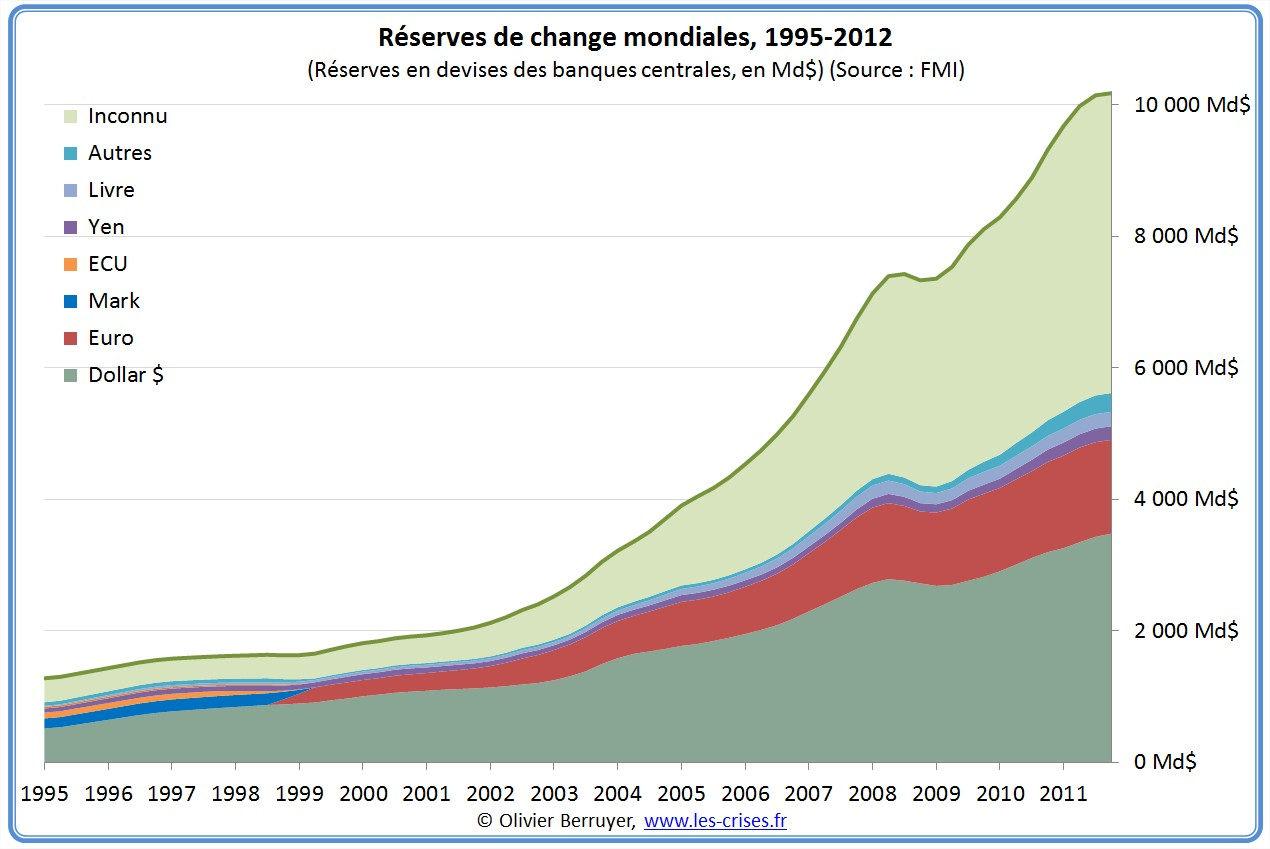
\includegraphics[width=0.8\textwidth]{res_mon.jpg}
        \end{minipage}
        \medskip

        \center
        \begin{tabular}{|*{4}{c|}}
               \hline
               & Dollar & Euro & Yen \\
               \hline
               Transactions sur le marché des changes & 44\% & 17\% & 11\% \\
               \hline
               Nombre de monnaies ancrées & 72\% & 26\% & 1\% \\
               \hline
               Prêts bancaires & 57\% & 20\% & 3\% \\
               \hline
               Obligations internationales & 39\% & 38\% & 3\% \\
               \hline
               Réserves officielles mondiales & 61\% & 24\% & 4\% \\
               \hline
        \end{tabular}
        \captionof{table}{Rôle international du dollar, de l'euro et du yen}
        \label{tab:title}

        \bigskip

        Cela peut s'expliquer par une forte inertie monétaire, mais aussi par le \emph{leadership politique} des États Unis, symbole du capitalisme. Le système politique de la monnaie est puissant, celui de l'euro est beaucoup plu faible. Du point de vue technique on retrouve aussi
        \begin{itemize}
                \item Faible signification des fluctuations et du taux de change.
                \item Coûts de change très élevés pour les entreprises. Par exemple Airbus, symbole de la réussite européenne ne travaille qu'avec des dollars.
                \item Coûts de transaction sur les marchés financiers européens plus élevés qu'aux États Unis.
                \item Incertitudes sur les rendements futurs des actifs européens.
                \item Politique \emph{contra-cyclique} de la BCE trop limitée par rapport à la FED.
        \end{itemize}
\end{document}
